\section{Fonctionnement des Protocoles Wi-Fi}
\label{sec:protocoles}

La sécurité des réseaux Wi-Fi repose sur une succession de mécanismes cryptographiques introduits progressivement pour corriger les vulnérabilités de leurs prédécesseurs. Depuis WEP en 1997 jusqu'à WPA3 en 2018, chaque protocole a apporté des évolutions majeures : nouveaux algorithmes, nouvelles primitives cryptographiques, mécanismes d'intégrité plus robustes, protection des trames de gestion, et résistance accrue aux attaques hors ligne. Cette section propose une analyse approfondie de ces mécanismes, de leur logique interne, de leurs limites, ainsi que des structures de trames qu'ils manipulent.

%%%%%%%%%%%%%%%%%%%%%%%%%%%%%%%%%%%%%%%%%%%%%%%%%%%%%%%%%%%%%%%%%%%%%%%%%%%%%%%%
% WEP
%%%%%%%%%%%%%%%%%%%%%%%%%%%%%%%%%%%%%%%%%%%%%%%%%%%%%%%%%%%%%%%%%%%%%%%%%%%%%%%%
\subsection{WEP : Wired Equivalent Privacy}

WEP (1997) constitue la première tentative de sécuriser les communications Wi-Fi. Il a été conçu à une époque où la cryptographie grand public était encore émergente, et souffre aujourd'hui de nombreuses limitations structurelles. Son objectif était de fournir une confidentialité comparable à celle d'un réseau filaire, mais son architecture s'est révélée profondément vulnérable.

\subsubsection*{Fonctionnement interne}

WEP repose sur l'algorithme de chiffrement par flot RC4. Le mécanisme de chiffrement est simple :
\begin{itemize}
    \item une clé secrète partagée statique (40 ou 104 bits) ;
    \item un vecteur d'initialisation (IV) de 24 bits, envoyé en clair ;
    \item concaténation \texttt{IV || clé} comme entrée du KSA de RC4 ;
    \item un ICV (Integrity Check Value) calculé via CRC-32, ajouté au plaintext avant chiffrement.
\end{itemize}

Le chiffrement d'un paquet se fait ainsi :

\begin{figure}[H]
\centering
\begin{tikzpicture}[node distance=2cm]
\node[draw, rounded corners, inner sep=3pt] (pt) {Plaintext + CRC-32};
\node[draw, rounded corners, right=of pt, inner sep=3pt] (iv) {IV (24 bits)};
\node[draw, rounded corners, below=of iv, inner sep=3pt] (rc4) {RC4 KSA/PRGA};
\node[draw, rounded corners, right=of rc4, inner sep=3pt] (ks) {Keystream};
\node[draw, rounded corners, right=of pt, yshift=-10mm, inner sep=3pt] (xor) {XOR};
\node[draw, rounded corners, right=of xor, inner sep=3pt] (ct) {Ciphertext};

\draw[->] (pt) -- (xor);
\draw[->] (iv) -- (rc4);
\draw[->] (rc4) -- (ks);
\draw[->] (ks) -- (xor);
\draw[->] (xor) -- (ct);

\end{tikzpicture}
\caption{Principe du chiffrement WEP}
\label{fig:wep}
\end{figure}

\paragraph{Format d'une trame WEP}

\begin{figure}[H]
\centering
\begin{tikzpicture}
\node[draw, minimum width=3cm] (hdr) {802.11 Header};
\node[draw, right=0cm of hdr, minimum width=2cm] (iv) {IV};
\node[draw, right=0cm of iv, minimum width=4cm] (data) {Données chiffrées};
\node[draw, right=0cm of data, minimum width=2cm] (icv) {ICV (CRC-32)};
\end{tikzpicture}
\caption{Format d'une trame WEP}
\end{figure}

\paragraph{Faiblesses cryptographiques majeures}

\begin{itemize}
    \item IV de 24 bits : collisions quasi certaines en quelques minutes.
    \item RC4 présente des biais initiaux exploités par les attaques FMS, KoreK et PTW.
    \item CRC-32 n'est pas une fonction d'intégrité cryptographique : vulnérable au bit-flipping.
    \item Pas de renouvellement de clé : longue exposition.
\end{itemize}

Ces vulnérabilités rendent WEP totalement compromis : casser une clé WEP prend moins d'une minute dans des conditions favorables.

%%%%%%%%%%%%%%%%%%%%%%%%%%%%%%%%%%%%%%%%%%%%%%%%%%%%%%%%%%%%%%%%%%%%%%%%%%%%%%%%
% WPA
%%%%%%%%%%%%%%%%%%%%%%%%%%%%%%%%%%%%%%%%%%%%%%%%%%%%%%%%%%%%%%%%%%%%%%%%%%%%%%%%
\subsection{WPA : Wi-Fi Protected Access}

Face à la crise WEP, la Wi-Fi Alliance introduit en 2003 WPA comme correctif transitoire, visant à remplacer les composants vulnérables tout en conservant le matériel existant (compatibilité ascendante).

\subsubsection*{Fonctionnement interne}

WPA introduit plusieurs mécanismes :
\begin{itemize}
    \item un mélange de clés élaboré (phase 1 et phase 2) ;
    \item un compteur TSC (TKIP Sequence Counter) antipiratage ;
    \item un MIC (Message Integrity Code) ;
    \item une rotation des clés fréquente.
\end{itemize}

Bien que RC4 soit toujours utilisé, WPA réduit significativement les risques d'attaque sans néanmoins les éliminer.

%%%%%%%%%%%%%%%%%%%%%%%%%%%%%%%%%%%%%%%%%%%%%%%%%%%%%%%%%%%%%%%%%%%%%%%%%%%%%%%%
% WPA2
%%%%%%%%%%%%%%%%%%%%%%%%%%%%%%%%%%%%%%%%%%%%%%%%%%%%%%%%%%%%%%%%%%%%%%%%%%%%%%%%
\subsection{WPA2 : AES-CCMP et le 4-Way Handshake}

WPA2 apporte une amélioration profonde : l’abandon de RC4 au profit d’un chiffrement moderne AES-CCMP.

\subsubsection*{Modes d’authentification}
\begin{itemize}
    \item \textbf{WPA2-PSK} : la PMK = PBKDF2(passphrase, SSID).
    \item \textbf{WPA2-Enterprise} : PMK fournie via un serveur RADIUS et une authentification EAP.
\end{itemize}

%%%%%%%%%%%%%%%%%%%%%%%%%%%%%%%%%%%%%%%%%%%%%%%%%%%%%%%%%%%%%%%%%%%%%%%%%%%%%%%%
% 4-Way Handshake
%%%%%%%%%%%%%%%%%%%%%%%%%%%%%%%%%%%%%%%%%%%%%%%%%%%%%%%%%%%%%%%%%%%%%%%%%%%%%%%%
\subsubsection*{Le 4-Way Handshake}

Le handshake assure :
\begin{itemize}
    \item la preuve de possession mutuelle de la PMK ;
    \item la génération de la PTK ;
    \item la distribution de la GTK.
\end{itemize}

\begin{figure}[H]
\centering
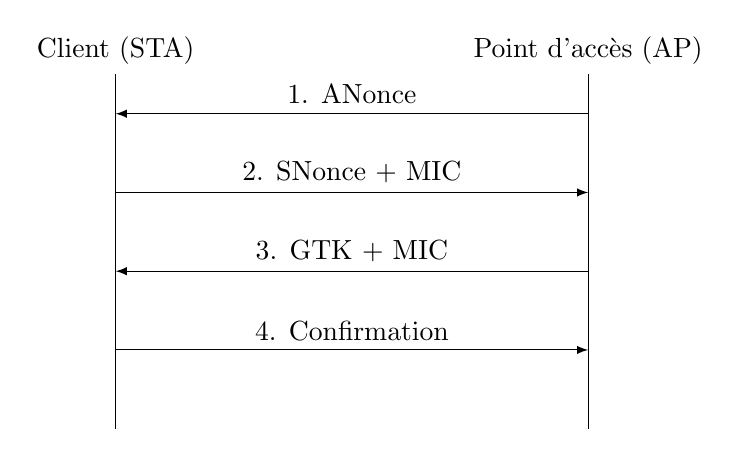
\begin{tikzpicture}[>=latex]

\node (sta) at (0,0) {Client (STA)};
\node (ap)  at (6,0) {Point d'accès (AP)};

\draw (sta.south) -- ++(0,-4.5);
\draw (ap.south)  -- ++(0,-4.5);

\draw[->] (ap.south)++(0,-0.5) -- node[above,sloped]{1. ANonce} ++(-6,0);
\draw[->] (sta.south)++(0,-1.5) -- node[above,sloped]{2. SNonce + MIC} ++(6,0);
\draw[->] (ap.south)++(0,-2.5) -- node[above,sloped]{3. GTK + MIC} ++(-6,0);
\draw[->] (sta.south)++(0,-3.5) -- node[above,sloped]{4. Confirmation} ++(6,0);

\end{tikzpicture}
\caption{4-Way Handshake WPA/WPA2}
\label{fig:4way}
\end{figure}

%%%%%%%%%%%%%%%%%%%%%%%%%%%%%%%%%%%%%%%%%%%%%%%%%%%%%%%%%%%%%%%%%%%%%%%%%%%%%%%%
% PMK -> PTK -> GTK derivation
%%%%%%%%%%%%%%%%%%%%%%%%%%%%%%%%%%%%%%%%%%%%%%%%%%%%%%%%%%%%%%%%%%%%%%%%%%%%%%%%
\subsection{Dérivation des clés : PMK, PTK et GTK}

\begin{figure}[H]
\centering
\begin{tikzpicture}[>=latex, node distance=1.8cm]

\node[draw, rounded corners, inner sep=4pt] (pmk) {PMK};
\node[draw, rounded corners, below=of pmk, inner sep=4pt] (prf) {PRF(PMK, nonces, MAC)};
\node[draw, rounded corners, below=of prf, inner sep=4pt] (ptk) {PTK = KCK || KEK || TK};
\node[draw, rounded corners, right=3cm of ptk, inner sep=4pt] (gtk) {GTK};

\draw[->] (pmk) -- (prf);
\draw[->] (prf) -- node[left]{4-way handshake} (ptk);
\draw[->] (ptk.east) -- node[above]{KEK} (gtk.west);

\end{tikzpicture}
\caption{Dérivation cryptographique PMK $\rightarrow$ PTK $\rightarrow$ GTK}
\end{figure}

%%%%%%%%%%%%%%%%%%%%%%%%%%%%%%%%%%%%%%%%%%%%%%%%%%%%%%%%%%%%%%%%%%%%%%%%%%%%%%%%
% CCMP frame format
%%%%%%%%%%%%%%%%%%%%%%%%%%%%%%%%%%%%%%%%%%%%%%%%%%%%%%%%%%%%%%%%%%%%%%%%%%%%%%%%
\subsubsection*{Format d'une trame CCMP (WPA2)}

\begin{figure}[H]
\centering
\begin{tikzpicture}
\node[draw, minimum width=3cm] (hdr) {802.11 Header};
\node[draw, minimum width=2cm, right=0cm of hdr] (pn) {PN};
\node[draw, minimum width=2cm, right=0cm of pn] (ccmp) {CCMP Header};
\node[draw, minimum width=4cm, right=0cm of ccmp] (data) {Payload (AES-CTR)};
\node[draw, minimum width=3cm, right=0cm of data] (mic) {MIC (CBC-MAC)};
\end{tikzpicture}
\caption{Structure d'une trame CCMP}
\end{figure}

%%%%%%%%%%%%%%%%%%%%%%%%%%%%%%%%%%%%%%%%%%%%%%%%%%%%%%%%%%%%%%%%%%%%%%%%%%%%%%%%
% WPA3 / SAE
%%%%%%%%%%%%%%%%%%%%%%%%%%%%%%%%%%%%%%%%%%%%%%%%%%%%%%%%%%%%%%%%%%%%%%%%%%%%%%%%
\subsection{WPA3 : SAE, Dragonfly, GCMP et PMF}

WPA3 corrige des failles structurelles de WPA2, notamment KRACK, en introduisant SAE (Dragonfly), OWE, PMF obligatoire, et le support obligatoire de GCMP dans certaines suites.

\subsubsection*{Handshake SAE (Dragonfly)}

\begin{figure}[H]
\centering
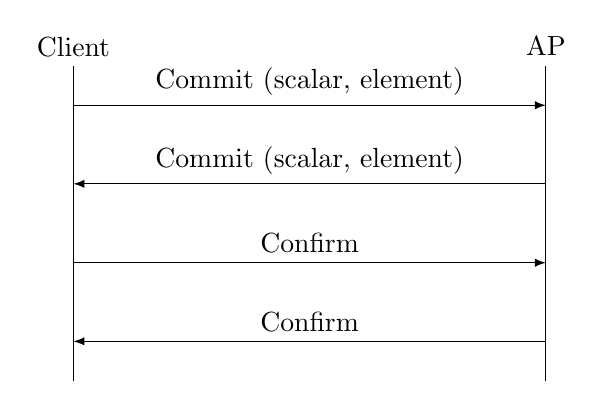
\begin{tikzpicture}[>=latex]

\node (sta) at (0,0) {Client};
\node (ap)  at (6,0) {AP};

\draw (sta.south) -- ++(0,-4);
\draw (ap.south)  -- ++(0,-4);

\draw[->] (sta.south)++(0,-0.5) -- node[above,sloped]{Commit (scalar, element)} ++(6,0);
\draw[->] (ap.south)++(0,-1.5) -- node[above,sloped]{Commit (scalar, element)} ++(-6,0);
\draw[->] (sta.south)++(0,-2.5) -- node[above,sloped]{Confirm} ++(6,0);
\draw[->] (ap.south)++(0,-3.5) -- node[above,sloped]{Confirm} ++(-6,0);

\end{tikzpicture}
\caption{Handshake SAE (WPA3)}
\end{figure}

%%%%%%%%%%%%%%%%%%%%%%%%%%%%%%%%%%%%%%%%%%%%%%%%%%%%%%%%%%%%%%%%%%%%%%%%%%%%%%%%
% SAE / GCMP crypto details
%%%%%%%%%%%%%%%%%%%%%%%%%%%%%%%%%%%%%%%%%%%%%%%%%%%%%%%%%%%%%%%%%%%%%%%%%%%%%%%%
\subsection{Mécanismes cryptographiques avancés}

Les protocoles de sécurité modernes du Wi-Fi reposent sur des mécanismes cryptographiques plus élaborés que ceux utilisés par les générations précédentes. Contrairement à WEP et TKIP, qui n’offraient qu’une protection minimale contre l’écoute, l’injection ou la manipulation des trames, WPA2 et surtout WPA3 reposent sur des constructions cryptographiques complètes, conçues pour fournir à la fois confidentialité, intégrité, résistance aux attaques par rejeu et garanties formelles sur la sécurité de la session. Trois mécanismes occupent une place centrale : AES-CCMP, GCMP et SAE (aussi appelé Dragonfly). Ces primitives ne jouent pas le même rôle, mais constituent ensemble la base de la sécurité Wi-Fi contemporaine.

\subsubsection{AES-CCMP}

AES-CCMP est devenu la norme de chiffrement par défaut avec WPA2. Son objectif est d’aller bien au-delà du simple masquage des données transportées : il assure simultanément la confidentialité des informations, l’intégrité des trames et la protection contre les attaques par rejeu.

Pour y parvenir, CCMP combine deux éléments complémentaires. D’une part, il utilise AES en mode compteur (CTR) pour le chiffrement. Ce mode transforme le bloc AES en générateur de flot chiffrant, permettant de chiffrer efficacement des paquets de taille variable sans introduire de structure exploitable. De l’autre, CCMP associe ce chiffrement à un code d’authentification basé sur CBC-MAC, un mécanisme cryptographique destiné à garantir que les données n’ont subi aucune altération. Cette combinaison forme une construction dite \textit{AEAD} (Authenticated Encryption with Associated Data), dans laquelle confidentialité et intégrité sont assurées simultanément par une même clé, ce qui évite un grand nombre de vulnérabilités présentes dans les générations antérieures.

L’ensemble repose également sur un numéro de paquet (Packet Number, PN) utilisé comme nonce unique. Toute réutilisation est interdite, ce qui empêche un attaquant de rejouer ou de réinjecter des trames chiffrées. En pratique, AES-CCMP constitue encore aujourd’hui une référence en matière de chiffrement pour les réseaux Wi-Fi.

AES-CCMP combine :
\begin{itemize}
    \item AES en mode CTR pour le chiffrement ;
    \item CBC-MAC pour l'intégrité (authentification).
\end{itemize}
C'est une construction AEAD robuste, largement testée.

\subsubsection{GCMP (AES-GCM)}

GCMP, introduit avec les standards 802.11ac et repris dans WPA3-Enterprise, reprend les principes d’AES-CCMP mais s’appuie cette fois sur AES-GCM. Cette construction fait partie des modes de chiffrement AEAD les plus étudiés et les plus robustes. AES-GCM associe un chiffrement en mode CTR à la fonction d’authentification GHASH, reposant sur des opérations arithmétiques dans un corps de Galois. Cette approche permet de calculer l’intégrité et le chiffrement de façon quasi parallèle, ce qui rend GCMP particulièrement performant sur les architectures modernes.

L’intérêt principal de GCMP réside donc dans sa rapidité : il offre un débit supérieur à CCMP, ce qui le rend bien adapté aux environnements à forte charge ou aux réseaux professionnels nécessitant des débits élevés. Il reste néanmoins sensible aux erreurs d’implémentation, comme l’ont montré certaines variantes des attaques Dragonblood qui ciblaient directement GCMP-128 lorsque les nonces n’étaient pas utilisés correctement. Malgré cela, GCMP demeure une brique cryptographique robuste lorsqu’il est correctement mis en œuvre.

\subsubsection{SAE / Dragonfly}


Contrairement à AES-CCMP et à GCMP, qui sont des mécanismes de chiffrement et d’intégrité utilisés \emph{après} l’établissement de la connexion, SAE (Simultaneous Authentication of Equals) intervient au moment de l’authentification. SAE n’est pas un algorithme de chiffrement mais un protocole d’échange de clés sécurisé, faisant partie de la famille des PAKE (Password-Authenticated Key Exchange).

L’enjeu de SAE est de résoudre l’un des problèmes fondamentaux des versions antérieures : avec WPA2-PSK, un attaquant pouvait capturer un 4-Way Handshake puis tenter hors ligne de retrouver le mot de passe par dictionnaire. Dans SAE, ce type d’attaque est impossible. Le protocole s'appuie sur un échange Diffie–Hellman (sur groupes modp ou courbes elliptiques), dans lequel le mot de passe n'est jamais transmis ni dérivé sous forme exploitable. Chaque tentative d’authentification nécessite une interaction en temps réel avec le point d’accès, ce qui empêche les attaques hors ligne et limite naturellement la vitesse des tests possibles.

SAE offre également la propriété de \textit{Forward Secrecy} : même si un mot de passe venait à être compromis ultérieurement, les sessions passées resteraient inexploitables, car la clé de session résulte d’un secret éphémère renouvelé à chaque connexion. Cette approche corrige l’une des failles conceptuelles les plus importantes de WPA2 et constitue la principale amélioration de WPA3-Personal.

Pour résumer, ses caractériques principales sont les suivantes :

\begin{itemize}
    \item s’appuie sur Diffie-Hellman (modp ou ECC) ;
    \item offre Forward Secrecy ;
    \item empêche les attaques hors-ligne ;
    \item protège contre attaques dictionnaires massives.
\end{itemize}

%%%%%%%%%%%%%%%%%%%%%%%%%%%%%%%%%%%%%%%%%%%%%%%%%%%%%%%%%%%%%%%%%%%%%%%%%%%%%%%%
% Format de trame GCMP
%%%%%%%%%%%%%%%%%%%%%%%%%%%%%%%%%%%%%%%%%%%%%%%%%%%%%%%%%%%%%%%%%%%%%%%%%%%%%%%%
\subsubsection*{Format d'une trame GCMP}

\begin{figure}[H]
\centering
\begin{tikzpicture}
\node[draw, minimum width=3cm] (hdr) {802.11 Header};
\node[draw, minimum width=2cm, right=0cm of hdr] (pn) {PN};
\node[draw, minimum width=2cm, right=0cm of pn] (gcmp) {GCMP Header};
\node[draw, minimum width=4cm, right=0cm of gcmp] (data) {Payload (AES-GCM)};
\node[draw, minimum width=3cm, right=0cm of data] (tag) {Tag (128 bits)};
\end{tikzpicture}
\caption{Structure d'une trame GCMP (WPA3)}
\end{figure}

%%%%%%%%%%%%%%%%%%%%%%%%%%%%%%%%%%%%%%%%%%%%%%%%%%%%%%%%%%%%%%%%%%%%%%%%%%%%%%%%
% Synthesis table
%%%%%%%%%%%%%%%%%%%%%%%%%%%%%%%%%%%%%%%%%%%%%%%%%%%%%%%%%%%%%%%%%%%%%%%%%%%%%%%%
\subsection{Synthèse comparative approfondie}

\begin{table}[H]
\centering
\begin{tabular}{|c|c|c|c|c|}
\hline
\textbf{Protocole} & \textbf{Crypto} & \textbf{Auth} & \textbf{Intégrité} & \textbf{Résistance} \\
\hline
WEP & RC4 & Clé statique & CRC-32 & Nulle \\
WPA & RC4 & PSK & MIC & Faible \\
WPA2 & AES-CCMP & PSK/802.1X & CBC-MAC & Forte (hors KRACK) \\
WPA3 & AES-CCMP/GCMP & SAE/802.1X & PMF & Très forte \\
OWE & Diffie-Hellman & Aucune & CCMP/GCMP & Élevée \\
\hline
\end{tabular}
\caption{Comparaison des protocoles de sécurité Wi-Fi}
\end{table}

\newpage